\chapter{实验结果及分析}
本章主要对本文提出的基于元学习本体增强的跨领域知识图谱表示模型(MOKER)进行实验的验证和效果的苹果。主要验证了该模型在面向跨设备情景下的测试数据集上的实验效果,并和目前已经提出的可以处理类似问题的归纳知识图谱表示模型的效果进行对比,结果显示该模型在引入多层次的特征信息后在实验数据上明显优于现有其他模型。最后通过对模型的多个消融实验也证明了模型各个部分的重要性。

\section{数据集}
由于传统的知识图谱数据集基本面向“closed-world”下的设定,即测试三元组中的关系和实体都是在训练三元组数据中已知的,不存在跨设备场景下的未见的组件,因此本文基于三个包含本体层面三元组的知识图谱DBpeida和NELL-995构建了包含未未知组件的新数据集DB\_Ext和NELL\_Ext对模型的效果进行测试,该三个数据集分别从经典的数据集DBpedia和NELL-995数据集中抽取部分子集得到。

\subsection{源数据集介绍}
DBpedia:DBpedia数据集是一个基于维基百科的语义知识库,该数据集由一个目前由一个开源社区维护并使用维基百科上的各种文章和各种在线网络资源进行扩展。DBpedia项目从wikipedia中提取结构化的数据,然后通过提取器将这些结构化的属性如图像、标签、描述文本等信息转化为事实三元组并进行存储,最新的数据集快照已经包含了8.5亿条事实三元组数据。除了丰富的事实三元组外,DBpedia强调按照本体论构建知识库,其本体类型数达到了768个类别,主要包含人物、地点、工作、组织等本体类型。这些实体、属性和关系通常以RDF图的形式进行存储,并以SPARQL作为标准查询语言。同时该开源社区提供了网页公布数据集最新的版本和统计数据,同时支持数据集各版本检索和下载,非常便于研究者使用。

NELL-995:NELL-995数据集是从NELL数据集中抽取用于知识图谱补全任务的一个基准数据集,NELL(Never Ending Language Learning)是一个由卡内基梅隆大学主导的自动化学习系统,用于从网络中的非结构文本中自动的提取知识。NELL-995数据集建立在NELL知识库上,包含995个实体和129个关系,涵盖了广泛的领域,如地理、医学、体育、音乐和文化等。NELL-995数据集具有对实体和关系进行细粒度类型分类的属性。每个实体都被分配到一组多层次的关系类型中,并且与其他实体之间的关系也相应地被分类。因此,NELL-995数据集是学习细粒度知识表示和关系推理模型的理想数据集。

\subsection{任务数据集构建}
为了抽取出包含未知组件组件的数据子集,本文首先将源数据集所有的三元组构建一个大的实体知识图谱,然后随机选取100个根实体节点各延伸10个相邻接点构成测试子图并从子图中的关系和实体中抽取1/10的关系和实体标记为测试集专属,从训练集中剔除这些专属的三元组从而构建出未见的组件。除此之外,为了专门测试模型对未见关系及未见实体的单独表示性能,在测试集中的query集设置中,本文将测试三元组分为三类,分别只包含了一种单独的未见组件及同时包含两种未见组件的query三元组部分。最终每个数据集中都包含了两个基本的子知识图谱\(\mathcal{G}^{train}\)和\(\mathcal{G}^{test}\),训练知识图谱和测试图谱都单独从标准知识图谱中抽取,其中测试图谱中的三元组包含了训练图谱中不存在的实体和关系。同时将测试图谱的测试三元组分为了三类:1、所有测试三元组中只包含了未见的实体(unseen\_ent);2、所有测试三元组中只包含了未见的关系(unseen\_rel);3、所有测试三元组中同时包含了未见的实体和关系(unseen\_both)。该测试数据集中的统计数据由下表所示。其中DB\_Ext数据集包含的测试三元组数量仅含未见的实体的三元组243个,仅含未见的关系的三元组10个,同时包含两个未见组件的三元组243个;NELL\_Ext数据集包含的测试三元组数量仅含未见的实体的三元组565个,仅含未见的关系的三元组12个,同时包含两个未见组件的三元组115个。

\subsection{数据集本体三元组获取}
为了获得知识图谱相关的本体三元组数据,在现存的可找到的本体三元组数据的基础上,本文扩展了类型相关的三元组数据,首先根据所有实体三元组的数据上映射到实体的类型信息,那么对于知识图谱中的所有关系来说,(type,relation,type)类型三元组中的type头结点即为关系在本体层次上的domain关系,type为结点即为关系在本体层次上的range关系,同时在进行构建的过程中本文根据type元关系出现的频率进行阈值的把控。除了根据type构建的本体三元组本文还引入了关系与关系的联系和type本身的本体三元组中的isa、synonym关系共同设置为generalizations关系加入到本体三元组数据中,最终构建出了由domain、range、generalizations三种元关系构成的本体三元组数据。其中三元组的统计数量如下表~\ref{tab:4-1}所示。
\begin{table}[h]
  \caption{数据集统计数据(括号中为未见组件数量)}
  \label{tab:4-1}
  \resizebox{\textwidth}{!}{%
  \begin{tabular}{cccccccc}
  \hline
                      & \multicolumn{3}{c}{训练图谱}                                                                                    & \multicolumn{4}{c}{测试图谱}                                                                                                                                                         \\ \cline{2-8} 
  \multirow{-2}{*}{} & 实体数                         & 关系数                        & 三元组数                                             & 实体数                             & 关系数                            & \begin{tabular}[c]{@{}c@{}}support\\ 三元组数\end{tabular} & \begin{tabular}[c]{@{}c@{}}query\\ 三元组数\end{tabular} \\ \hline
  NELL\_Ext          & {\color[HTML]{333333} 1583} & {\color[HTML]{333333} 153} & \multicolumn{1}{c|}{{\color[HTML]{333333} 5269}} & {\color[HTML]{333333} 851(753)} & {\color[HTML]{333333} 140(30)} & {\color[HTML]{333333} 2160}                            & {\color[HTML]{333333} 692}                           \\
  DB\_Ext            & {\color[HTML]{333333} 795}  & {\color[HTML]{333333} 115} & \multicolumn{1}{c|}{{\color[HTML]{333333} 1508}} & {\color[HTML]{333333} 913(884)} & {\color[HTML]{333333} 128(46)} & {\color[HTML]{333333} 1930}                            & {\color[HTML]{333333} 496}                           \\ \hline
  \end{tabular}%
  }
  \end{table}

\section{实验设计及评价指标}
本实验包含本体嵌入表示学习和未见组件表示学习两个阶段,第一个阶段主要学习到融合描述文本信息的本体嵌入表示,第二阶段使用本体信息进行未见组件的表示学习。

第一阶段首先采用传统的表示学习方法对本体三元组数据进行初步嵌入表示;然后对本体节点的描述信息从预训练词嵌入glove中获得各描述文本单词的初始化词向量,使用TF-IDF统计方法判断单词的重要程度对各单词的词向量进行加权聚合计算获得本体节点描述文本的初始化向量嵌入;最后本体三元组的结构化表示嵌入和本体描述文本的表示嵌入映射到同一个空间中进行评分和更新,获得拼接后的最终的本体嵌入。

第二阶段对未见组件进行表示学习,为了在元学习中模拟出存在未见组件的场景,在每个元学习任务的设置中都人为抹除了一些实体和关系的标签,使得这些实体和关系必须通过的模型学习得到嵌入表示而不是从传统嵌入方法的嵌入矩阵中取得,具体的一个task实验流程如下:
\begin{enumerate}[label=\arabic*)]
  \item 从训练数据集中随机挑选任意10个起始节点,然后根据这10个起始节点的关系延伸出邻居节点补充到子图中。
  \item 每次选取64个子图组成一个batch进行一个task任务的训练。
  \item 通过模型获得这个batch的关系表示和节点表示。
  \item 计算batch单个子项的loss和整个batch的loss。
  \item 根据loss进行梯度下降求解最优参数。
\end{enumerate}
对于模型在链接预测任务上的评价指标,本文选取了MRR和Hit@10作为评判的标准。其中MRR通过计算预测三元组排名的倒数来进行计算,即对测试三元组中的所有事实三元组,如果该三元组在预测排名中得分高那么排名就靠前,对应的倒数也会比较大,因此MRR作为评价指标越大则证明总体链接预测的排名较好。而Hits@n指的是在预测三元组中排名小于n的三元组的平均占比,计算公式如下:
\begin{equation}
  HITS@n = \frac{1}{|S|} \sum_{i=1}^{|S|}||(rank_{i} \leqslant n) \label{eq:4-1}
\end{equation}

假如n设置为10,那么统计事实三元组在预测三元组中前n名的个数,最后再除以总个数就得到了Hits@10的结果,其中\(||(·)\)为indicator函数(若条件真则函数值为1,否则为0)。

参与比较的模型如下:

GraIL:不直接学习实体节点对应的嵌入也没有使用任何节点的属性,而是在测试三元组候选关系的周围构建子图,通过子图的结构和结构化的节点特征来对三元组进行预测,使得模型能够很好的作用在未知的实体三元组预测任务上。

CoMPILE:对GraIL模型的子图归纳模型进行了改进,加强了对子图关系方向性的限制,同时在对未知节点特征聚合的信息传递过程中增加了先前模型中忽略的关系特征。

DURM:提出一个可同时学习规则逻辑及其置信度得分方法的可微模型,并且可以使用梯度优化的方法来优化归纳逻辑编程任务,可用于处理含有未知实体的链接预测任务。

Neural-LP:基于知识库构建一个可学习逻辑规则的可微模型,因为逻辑规则是独立于实体和关系的,因此理论上可作用在任何未见的实体上,在归纳图谱补全任务上相比于传统的对实体进行结构信息表示学习的方法有很大提升。

MaKEr:通过对关系结构的特征学习聚合关系邻接关系的特征对关系进行表示,聚合关系特征对实体编码,借用拓扑结构的信息一定程度上实现对未见实体和未见关系表示。

\section{模型参数设置}
对于用于对比的baseline模型的参数设置,本文遵循了相关论文给出的最优超参数设置,对于本文提出的模型的相关参数设置如下表\ref{tab:4-2}所示:
\begin{table}[h]
  \caption{模型超参数设置}
  \label{tab:4-2}
  \resizebox{\textwidth}{!}{%
  \begin{tabular}{|c|c|c|c|c|c|}
  \hline
  {\color[HTML]{333333} 本体嵌入参数}           & {\color[HTML]{333333} 设置值}     & {\color[HTML]{333333} 元学习训练参数}                          & {\color[HTML]{333333} 设置值}    & {\color[HTML]{333333} 嵌入参数}        & {\color[HTML]{333333} 元学习训练参数} \\ \hline
  {\color[HTML]{333333} lr}               & {\color[HTML]{333333} 0.00005} & {\color[HTML]{333333} lr}                               & {\color[HTML]{333333} 0.001}  & {\color[HTML]{333333} dim}         & {\color[HTML]{333333} 300}     \\ \hline
  {\color[HTML]{333333} ent\_str\_dim}    & {\color[HTML]{333333} 150}     & {\color[HTML]{333333} train\_bs}                        & {\color[HTML]{333333} 64}     & {\color[HTML]{333333} num\_gcn}    & {\color[HTML]{333333} 2}       \\ \hline
  {\color[HTML]{333333} ent\_text\_dim}   & {\color[HTML]{333333} 300}     & {\color[HTML]{333333} eval\_bs}                         & {\color[HTML]{333333} 16}     & {\color[HTML]{333333} num\_comgcn} & {\color[HTML]{333333} 2}       \\ \hline
  {\color[HTML]{333333} mapping\_size}    & {\color[HTML]{333333} 300}     & {\color[HTML]{333333} num\_step}                        & {\color[HTML]{333333} 100000} & {\color[HTML]{333333} gcn\_dim}    & {\color[HTML]{333333} 300}     \\ \hline
  {\color[HTML]{333333} training\_epochs} & {\color[HTML]{333333} 1000}    & {\color[HTML]{333333} early\_stop\_patience}            & {\color[HTML]{333333} 20}     & {\color[HTML]{333333} hid\_drop}   & {\color[HTML]{333333} 0.3}     \\ \hline
  {\color[HTML]{333333} batch\_size}      & {\color[HTML]{333333} 100}     & {\color[HTML]{333333} num\_sample\_for\_estimate\_size} & {\color[HTML]{333333} 10}     & {\color[HTML]{333333} -}           & {\color[HTML]{333333} -}       \\ \hline
  \end{tabular}%
  }
\end{table}

其中主要包含一下三个方面的参数设置:
\begin{enumerate}[label=\arabic*)]
\item 在本体三元组进行嵌入时模型学习率lr、本体三元组概念节点结构嵌入维度ent\_str\_dim、本体概念节点文本嵌入维度ent\_text\_dim、线性隐藏层维度mapping\_size以及训练的epoch数量和batch的大小。
\item 对知识图谱表示元学习训练相关的任务学习率lr、单任务支持集的batch数量train\_bs、单任务查询集的batch数量eval\_bs、元训练总任务数num\_step、元训练提前结束无效训练任务计数early\_stop\_patience以及单个batch采样的根节点数。
\item 对实体和关系嵌入基本维度的设置dim、关系位置图对关系进行GCN的层数num\_gcn、GCN中间传递维度gcn\_dim以及GCN层的丢弃率hid\_drop、对关系和实体进行联合学习的ComGCN的层数。
\end{enumerate}

在对三元组进行链接预测的评定过程中,本文通过对ComGCN第二层输出的改进可支持多种KGE模型作为评分函数,实际采用的KGE模型包含TransE、DistMult、ComplEx及RotatE,实体和关系的维度根据采用的KGE模型在基础嵌入维度上进行调整,具体如下表\ref{tab:4-3}所示:
\begin{table}[h]
  \caption{评分函数}
  \label{tab:4-3}
  \centering
  \resizebox{0.8\textwidth}{!}{%
  \begin{tabular}{|l|l|l|l|}
  \hline
  {\color[HTML]{333333} 模型名}      & {\color[HTML]{333333} 实体维度}    & {\color[HTML]{333333} 关系维度}    & {\color[HTML]{333333} 评分函数}                 \\ \hline
  {\color[HTML]{333333} TranE}    & {\color[HTML]{333333} dim}     & {\color[HTML]{333333} dim}     & {\color[HTML]{333333} F = -|| h + r - t ||} \\ \hline
  {\color[HTML]{333333} DistMult} & {\color[HTML]{333333} dim}     & {\color[HTML]{333333} dim}     & {\color[HTML]{333333} F = \(\rm h^{T}\) diag(r) t}     \\ \hline
  {\color[HTML]{333333} ComplEx}  & {\color[HTML]{333333} 2 * dim} & {\color[HTML]{333333} 2 * dim} & {\color[HTML]{333333} F = Re(\(\rm h^{T}\) diag(r) t)} \\ \hline
  {\color[HTML]{333333} RotatE}   & {\color[HTML]{333333} 2 * dim} & {\color[HTML]{333333} dim}     & {\color[HTML]{333333} F = -|| h ○ r - t ||} \\ \hline
  \end{tabular}%
  }
\end{table}

其中评分函数中的h、r、t分别指代头实体、关系和尾实体的嵌入表示,Re表示复向量的实部分量,○操作表示哈达玛积。

\section{实验结果及分析}
各模型在NELL\_Ext上的链接预测任务实验结果如下表\ref{tab:4-4}所示,按照测试数据集的三元组对未知组件的包含情况,分为了只包含未知实体的结果(u\_ent)、只包含未知关系的结果(u\_rel)以及同时包含未知实体和未见关系的结果(u\_both)。表格中加粗的为最优的实验效果,带有下划线则是该类基本模型中表现最优的得分,模型括号后面的指代的是在评分阶段采用的KGE评分函数。
\begin{table}[h]
  \caption{NELL\_Ext数据集结果}
  \label{tab:4-4}
  \resizebox{\textwidth}{!}{%
  \begin{tabular}{ccccccc}
  \hline
  \multicolumn{7}{c}{NELL\_Ext}                                                                                                                 \\ \hline
  \multicolumn{1}{l|}{\multirow{2}{*}{}} & \multicolumn{2}{c}{u\_ent}       & \multicolumn{2}{c}{u\_rel}       & \multicolumn{2}{c}{u\_both}      \\ \cline{2-7} 
  \multicolumn{1}{l|}{}                  & MRR            & Hits@10        & MRR            & Hits@10        & MRR            & Hits@10        \\ \hline
  \multicolumn{1}{c|}{Neural-LP}         & 30.48          & 47.96          & -              & -              & -              & -              \\
  \multicolumn{1}{c|}{DRUM}              & 31.82          & 48.32          & -              & -              & -              & -              \\
  \multicolumn{1}{c|}{GraIL}             & 71.62          & 92.92          & -              & -              & -              & -              \\
  \multicolumn{1}{c|}{CoMPILE}           & {\ul 75.94}    & {\ul 93.62}    & -              & -              & -              & -              \\ \hline
  \multicolumn{1}{c|}{MaKEr(TransE)}     & 70.82          & 92.00          & 24.56          & 54.17          & 21.53          & 51.74          \\
  \multicolumn{1}{c|}{MaKEr(DistMult)}   & 70.63          & 91.33          & 27.02          & 60.00          & \textbf{41.39} & 57.65          \\
  \multicolumn{1}{c|}{MaKEr(ComplEx)}    & 72.24          & 91.91          & 18.27          & 34.17          & 29.39          & 59.65          \\
  \multicolumn{1}{c|}{MaKEr(RotatE)}     & {\ul 77.09}    & {\ul 94.64}    & {\ul 31.53}    & {\ul 55.00}    & 31.45          & {\ul 62.35}    \\ \hline
  \multicolumn{1}{c|}{MOKER(TransE)}     & 78.28          & 94.86          & 20.72          & 53.34          & 27.11          & 55.85          \\
  \multicolumn{1}{c|}{MOKER(DistMult)}   & 75.98          & 92.46          & 19.30          & 22.50          & 31.37          & 55.65          \\
  \multicolumn{1}{c|}{MOKER(ComplEx)}    & 73.61          & 90.60          & 24.44          & 38.33          & 29.70          & 54.96          \\
  \multicolumn{1}{c|}{MOKER(RotatE)}     & \textbf{79.92} & \textbf{94.73} & \textbf{45.07} & \textbf{75.63} & {\ul 40.33}    & \textbf{67.06} \\ \hline
  \end{tabular}%
  }
  \end{table}
各模型在DB\_Ext上的链接预测任务实验结果如下表\ref{tab:4-5}所示:
\begin{table}[h]
  \caption{DB\_Ext数据集结果}
  \label{tab:4-5}
  \resizebox{\textwidth}{!}{%
  \begin{tabular}{ccccccc}
  \hline
  \multicolumn{7}{c}{DB\_Ext}                                                                                                                 \\ \hline
  \multicolumn{1}{l|}{}                & \multicolumn{2}{c}{u\_ent}       & \multicolumn{2}{c}{u\_rel}       & \multicolumn{2}{c}{u\_both}      \\ \cline{2-7} 
  \multicolumn{1}{l|}{}                & MRR            & Hits@10        & MRR            & Hits@10        & MRR            & Hits@10        \\ \hline
  \multicolumn{1}{c|}{Neural-LP}       & 57.15          & 73.46          & -              & -              & -              & -              \\
  \multicolumn{1}{c|}{DRUM}            & 59.88          & 73.25          & -              & -              & -              & -              \\
  \multicolumn{1}{c|}{GraIL}           & 59.44          & {\ul 80.86}    & -              & -              & -              & -              \\
  \multicolumn{1}{c|}{CoMPILE}         & {\ul 60.66}    & 79.93          & -              & -              & -              & -              \\ \hline
  \multicolumn{1}{c|}{MaKEr(TransE)}   & 54.4           & 83.7           & 31.13          & 54.00          & 38.66          & 66.5           \\
  \multicolumn{1}{c|}{MaKEr(DistMult)} & 46.24          & 81.07          & 16.43          & 11.00          & 32.16          & 56.71          \\
  \multicolumn{1}{c|}{MaKEr(ComplEx)}  & 53.79          & 82.47          & 19.95          & 29.00          & 36.88          & 59.26          \\
  \multicolumn{1}{c|}{MaKEr(RotatE)}   & {\ul 59.55}    & {\ul 86.09}    & {\ul 32.93}    & {\ul 55.00}    & \textbf{41.27} & {\ul 66.54}    \\ \hline
  \multicolumn{1}{c|}{MOKER(TransE)}   & 64.63          & 89.60          & \textbf{44.77} & 70.25          & 34.92          & \textbf{69.42} \\
  \multicolumn{1}{c|}{MOKER(DistMult)} & 56.73          & 80.25          & 13.68          & 11.00          & 33.94          & 61.74          \\
  \multicolumn{1}{c|}{MOKER(ComplEx)}  & 52.22          & 77.34          & 14.40          & 15.00          & 31.72          & 59.49          \\
  \multicolumn{1}{c|}{MOKER(RotatE)}   & \textbf{66.43} & \textbf{89.67} & 41.80          & \textbf{74.00} & {\ul 35.11}    & 63.81          \\ \hline
  \end{tabular}%
  }
\end{table}
上面两个表格展示了各模型在NELL\_Ext和DB\_Ext上的链接预测结果,其中Hits@10在计算的过程中本文选择了50个候选进行评估,并且根据不同类型的查询三元组(即u\_ent、u\_rel和u\_both)显示了不同的模型得分。而且对于GraIL、Neural-LP、DRUM和CoMPILE在对应的论文中只在包含未知实体的数据集上做了实验,因此在对存在未见关系的测试集结果上进行留空处理,但是仍在未见实体的测试集中比较相对应的效果。上述结果均为响应模型运行4此后取平均值的结果。

从结果中表明本文提出的模型MOKER相比于其他baseline模型有所改进且在不同的KGE评分模型上基本上有不同程度的提升,而且最优的结果基本上由MOKER与RotatE模型组合得出,RotatE模型相比于其他的KGE模型采用了更加复杂的关系和实体的映射关系因此能表现更多的没有重叠的特征信息,同时也证明了本文模型的有效性。

在处理未见的实体的测试集上,本文比较了基于规则学习处理未见实体的Neural-LP模型和DRUM模型以及基于子图推理的GraIL模型和CoMPILE模型。从结果上可以明显看出基于规则的模型依赖于针对数据集学习出的规则,模型效果受数据集影响较大,且需要有大量的数据集或者样本平衡要求十分严格,总体效果没有基于子图的模型效果好,在NELL\_Ext数据集上结果差距较大。CoMPILE模型在GraIL模型的基础上强调了关系的重要性,总体效果上要比GraIL表现更好。但上述四个模型首先无法处理未见关系,而且基于子图的归纳推理模型强调了测试三元组中头尾实体间的局部子图信息,没有完全利用到实体周围的结构特征信息以及关系信息。MaKEr模型虽然考虑到了关系对实体的重要性,但是在关系表示的特征学习上效果比本文模型要差,因此通过邻接关系聚合特征表示未知实体的效果在MRR的评价指标上比本文模型平均低了4.42\%,在Hits@10的表现上本文模型在对应RotatE评分函数上也领先了1.85\%,说明了本文模型在未见实体表示上的有效性。

在处理未见关系和同时处理两种未知组件的测试集上,本文比较了通过结构信息对关系进行编码并通过聚合关系信息对未见实体进行编码的MaKEr模型,对于未见的关系,本文通过引入额外的本体知识作为关系语义信息的补充,同时通过关系的位置结构利用GCN对关系的表示进行更新以学习到未见关系周围的结构拓扑信息。从两个数据集上的链接预测任务结果来看,相比于MaKEr模型仅学习结构信息对关系表示,本文引入的本体信息能够有效对关系的表示进行语义补充,在处理未见关系时RotatE模型中表现出明显的优势,其MRR得分比MaKEr的得分高14.54\%,而在Hits@10的得分方面,70.63的得分比MaKEr的得分高出20\%左右。表明本文模型能够更好地捕捉关系的语义和结构信息,在考虑局部和全局关系时都具有不错的性能。在同时含有两种未知组件的测试集上,相比于MaKEr模型,本文模型在NELL\_Ext数据集的Hits@10评分上有平均1.82\%的提升,在DB\_Ext数据集的MRR和Hits@10分别有平均1.18\%和0.53\%的提升。

除此之外,本文实验发现,TransE和RotatE的模型效果比DistMult和ComplEx模型更好,尤其在关系处理方面。在本体嵌入实验中,采用RotatE作为评分函数,对实体知识图谱进行表示。DistMult和ComplEx模型因其复杂性不适合与RotatE的本体嵌入配合,而效果反而下降。相比之下,TransE模型简洁易操作,在进行特征提取时更加适合。而RotatE作为近几年提出的KGE模型,一方面本身与本体嵌入方法相同,另一方面个更全面的对实体和关系进行低纬嵌入表示,因此取得了本文模型中的最优效果。

\section{模型消融实验}
本节将介绍针对模型的几个重要模块的多项消融实验,以展示本文模型的不同部分的重要性,主要设置了5项不同的消融设置实验:(1)去除元学习的设置;(2)去除本体的设置;(3)去除实体聚合表示的设置;(4)去除关系GCN聚合的设置;(5)同时去除本体和元学习的设置;获得的实验结果如表\ref{tab:4-6}所示:
\begin{table}[h]
  \caption{在NELL\_Ext上的消融实验结果}
  \resizebox{\textwidth}{!}{%
  \label{tab:4-6}
  \begin{tabular}{ccccccc}
  \hline
  \multicolumn{7}{c}{NELL\_Ext}                                                                                                                  \\ \hline
  \multicolumn{1}{l|}{}                   & \multicolumn{2}{c}{u\_ent}       & \multicolumn{2}{c}{u\_rel}       & \multicolumn{2}{c}{u\_both}      \\ \cline{2-7} 
  \multicolumn{1}{l|}{}                   & MRR            & Hits@10        & MRR            & Hits@10        & MRR            & Hits@10        \\ \hline
  \multicolumn{1}{c|}{MOKER(TransE)}      & \textbf{78.28} & \textbf{94.86} & 20.72          & 53.34          & \textbf{27.11} & \textbf{55.85} \\ \hline
  \multicolumn{1}{c|}{no\_meta\_TransE}     & 29.31          & 43.82          & 12.65          & 30.83          & 10.18          & 22.26          \\
  \multicolumn{1}{c|}{no\_ont\_TransE}      & 76.89          & 94.07          & 14.96          & 27.50          & 14.06          & 28.78          \\
  \multicolumn{1}{c|}{no\_ent\_TransE}      & 76.85          & 94.07          & 18.00          & 55.83          & 19.43          & 50.7           \\
  \multicolumn{1}{c|}{no\_gcn\_TransE}      & 74.68          & 92.27          & \textbf{23.88} & \textbf{61.67} & 19.85          & 46.26          \\
  \multicolumn{1}{c|}{no\_meta\_ont\_TransE} & 26.57          & 38.69          & 11.15          & 25.00          & 12.62          & 27.74          \\ \hline
  \end{tabular}%
  }
  \end{table}

其中个消融实验的具体设置如下:
\begin{enumerate}[label=\arabic*)]
  \item 去除元学习的设置:在模型训练阶段,本文采用了元学习的设置在训练集上提取任务子图并通过随机标签来模拟出未见的组件从而训练出模型处理未见组件的能力。在该消融实验下,取消掉了对子图标签的模拟效果即按照传统KGE模型的训练方法,在训练集上对所有三元组进行嵌入和损失计算。
  \item 去除本体的设置:本文模型的一个创新点即在对关系嵌入表示的时候通过关系位置图加入本体信息进行学习,在该消融实验设置下,将本体信息替换为随机表示对未见关系进行特征学习。
  \item 去除实体聚合表示的设置:本文模型在处理未见实体时,采用该实体周围的关系信息聚合表示,该消融实验设置下对未见实体进行随机化嵌入设置,考察未见实体的表示模块。
  \item 去除关系GCN聚合的设置:在构建完关系的位置图并引入本体嵌入后,本非模型通过GCN来加强关系对邻接结构的特征学习,该消融实验下去除两层GCN层,直接使用本体信息。
  \item 同时去除本体和元学习设置:同时结合消融实验(1)和(2)的设置。
\end{enumerate}

消融实验结果与MOKER(TransE)模型在NELL\_Ext上的实验结果进行比较,从消融实验结果可以看出,基本所有的消融设置都会导致性能下降,表明这些设计的重要性。但是在去除关系GCN聚合的设置上,在仅含有未见关系的测试集上效果反而提升,分析可知该层GCN的作用是在关系本体嵌入的基础上学习关系邻接关系的结构信息,这些结构信息的引入一定程度上会影响仅对关系的表示效果导致在仅包含未见关系的测试集上的效果下降。但是这些结构信息的引入在中未见实体的表示中,因为实体需要聚合邻接关系进行表示,因此引入的结构信息会对实体的表示效果进行提升,可以发现去掉GCN在包含未见实体和同时包含未见实体和未见关系的测试集上效果都有明显的下降,因此也侧面证明了GCN模型对实验效果提升的必要性。此外,本文观察到元学习设置对模型性能至关重要,表明在推广到测试知识图谱的任务上对模型进行元训练的有效性。

\section{未见实体案例分析}
在图\ref{fig:4-1}中展示了本体提出的MOKER模型和去除元学习和本体嵌入的传统TransE-KGE模型产生的在NELL-Ext数据集的测试集上实体嵌入的可视化。在这张图中,不同颜色展示了不同类型的实体,圆点代表未见的实体,叉号则代表了该类型下的已知实体。可以看出MOKER产生的嵌入分布与对应类型更加一致,在嵌入映射的距离上更近紧凑,而TransE-KGE产生的嵌入则混合了不同实体类型。MOKER将嵌入映射到了不同的聚类中,而TransE-KGE中不同实体类型的嵌入则混合在一起。此外,本文的模型可以将未见过的实体的嵌入与同一类型的已知实体聚类。不同类型实体的聚类表明,MOKER能够用包含合理语义和信息性知识的嵌入来表示未见过的实体。
\begin{figure}[h]
  \centering
  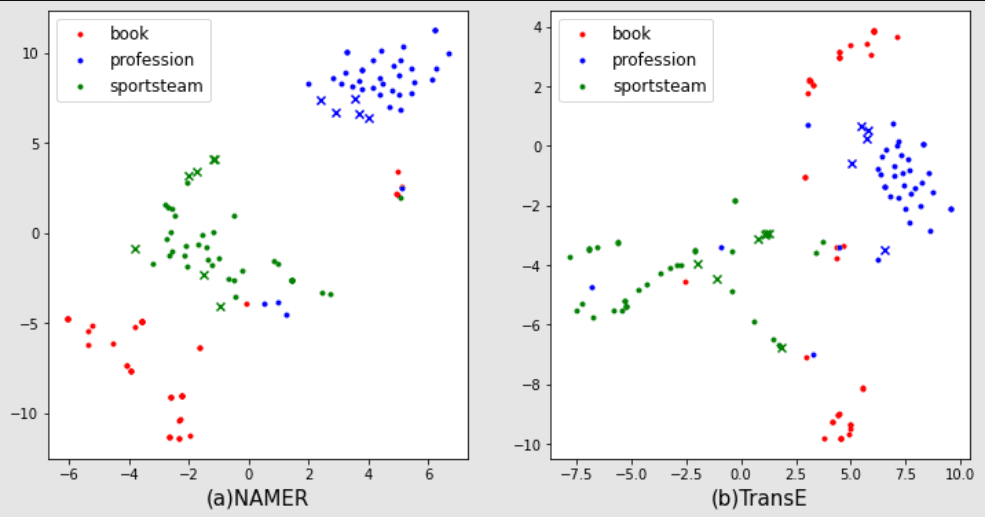
\includegraphics[width=0.8\textwidth]{4-1.png}
  \caption{实体嵌入可视化分析}
  \label{fig:4-1}
\end{figure}

\section{未见关系案例分析}
对于未见关系,本文选取了部分关系同样映射到了二维空间上进行可视化分析,如图\ref{fig:4-2}所示,其中圆点代表通过训练集中可见的关系,叉号代表测试集中的未见关系。本文模型通过采用关系位置图根据关系的相对位置对关系局部的邻接关系进行建模学习到了关系的拓扑结构信息,同时引入本体信息作为语义补充,因此同一实体的具有相近语义的相邻关系在距离上应该表现为更加相近,从图上可以看出,对于未见关系has\_office\_in\_city贴近于具有类似语义的关系has\_office\_in\_coutry,未见关系person\_born\_in\_city更贴近于已知关系person\_born\_in\_location。而对于已知关系parent\_of\_person和father\_of\_person和未见关系mother\_of\_person,本文可知一个实体如果存在parent\_of\_person的关系那么该实体节点的邻接关系中只能存在其中一个father或者mother的关系,因此在图中本文可以观察到mother\_of\_person在距离上更接近于parent\_of\_person关系,而远离father\_of\_person关系。由此可见,本文模型通过关系的位置图上联合本体语义信息有效的学习到了对应关系的语义关系,且其中相似的关系在向量空间中靠近,显示了本文提出的MOKER在嵌入未知关系方面的有效性。
\begin{figure}[h]
  \centering
  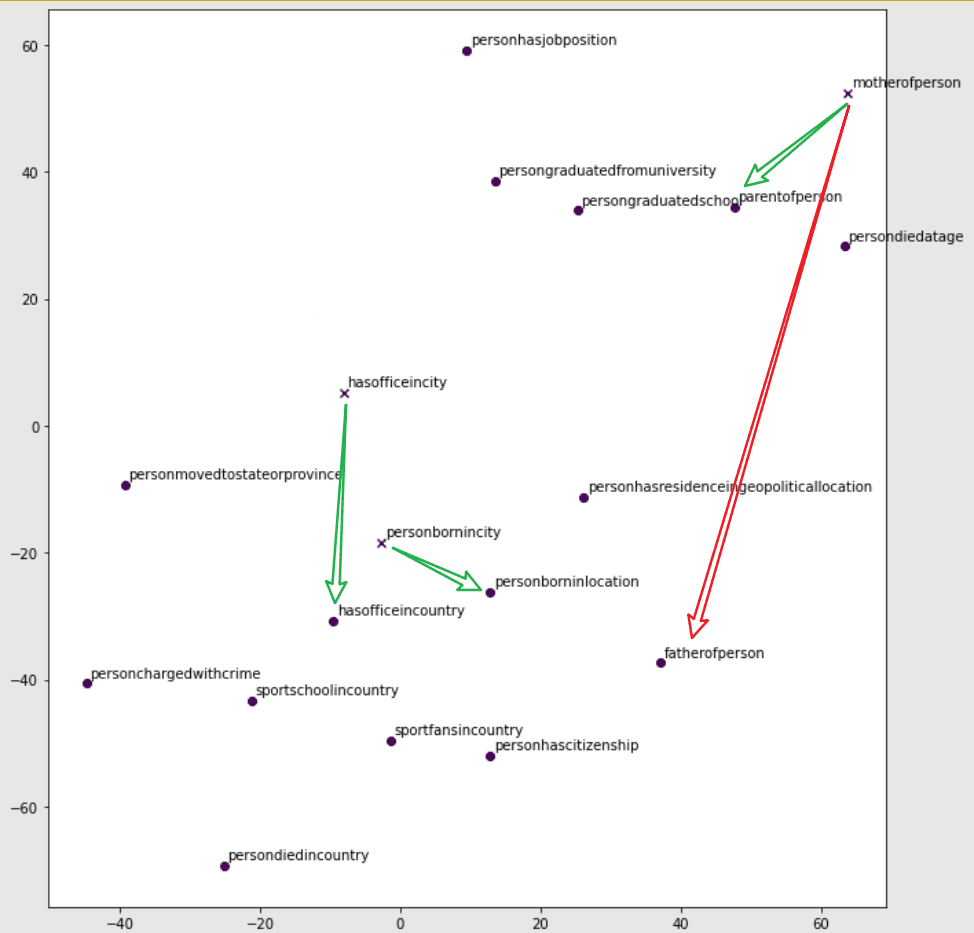
\includegraphics[width=0.9\textwidth]{4-2.png}
  \caption{实体嵌入可视化分析}
  \label{fig:4-2}
\end{figure}

\section{本章小结}
本章将本文提出的模型在测试数据集上NELL\_Ext和DB\_Ext上进行了链接预测任务的相关实验,测试数据集从NELL-995和DBpedia上抽取子集并添加了测试集中的未见组件。与多个基准模型相比,本文提出的模型在任务得分上均有不同程度的提升,并通过对实验结果的分析验证了模型对于表示学习效果增强的有效性。同时通过对各个模型组件的消融实验发现明显的效果下降,证明了模型模块的重要性;最后对未见实体和未见关系的案例分析可知得到的嵌入表示符合模型原理设定,再次证明了该模型对未见组件表示上的突出能力。